\section{Техническое задание}

\subsection{Основание для разработки}
Основанием для разработки является задание на выпускную квалификационную работу бакалавра по теме «Бизнес-проект \textquotedbl Разработка цифровой платформы Курский край\textquotedbl . Разработка веб-приложения».

\subsection{Цель и назначение разработки}
Целью разработки является создание программно-информационной системы, предоставляющей пользователям удобный интерактивный гид по городу Курску, а администратору --- инструменты управления контентом (объектами, категориями и маршрутами).

Для достижения указанной цели система должна покрывать как пользовательские сценарии навигации по городу, так и административные сценарии сопровождения контента.

\subsection{Требования к функциональности}
Информационная система должна обеспечивать выполнение следующих функций:
\begin{enumerate}
	\item \textbf{Управление объектами городской инфраструктуры.}
	Система должна предоставлять администратору возможность добавления новых объектов (достопримечательности, парки, кафе и другие категории), редактирования существующих карточек и удаления записей. Для каждого объекта должны поддерживаться координаты, краткое и подробное описание, контактная информация, главное изображение, галерея и признак публикации.
	
	\item \textbf{Категоризация и фильтрация контента.}
	Должна быть реализована работа со справочником категорий (создание новых категорий через административный интерфейс) и фильтрация пользовательского каталога по выбранной категории. Фильтрация должна выполняться без потери контекста просмотра и обеспечивать быстрый переход к карточке выбранного объекта.
	
	\item \textbf{Отображение объектов на интерактивной карте.}
	Система должна визуализировать опубликованные объекты на карте, поддерживать открытие карточки по маркеру и переход из карточки к фокусировке карты на выбранной точке.
	
	\item \textbf{Управление маршрутами.}
	Администратор должен иметь возможность создавать, редактировать и удалять маршруты, включая управление признаком публикации. Маршрут должен содержать не менее двух точек (старт и финиш), а также поддерживать добавление промежуточных точек и изменение их порядка.
	
	\item \textbf{Пользовательский просмотр маршрутов.}
	Пользовательская часть должна обеспечивать просмотр списка опубликованных маршрутов, открытие детальной карточки маршрута, отображение последовательности точек и визуализацию маршрута на карте.
	
	\item \textbf{Фотогалерея и связанный контент.}
	Система должна предоставлять отдельный раздел фото, открытие изображения в модальном окне и переход к связанному объекту из фото-интерфейса.
	
	\item \textbf{Доступ к административным функциям.}
	Административные функции должны быть доступны на выделенной странице управления контентом, включающей формы для объектов и маршрутов, таблицы текущих записей и инструменты быстрой модерации опубликованности.
\end{enumerate}

\subsection{Требования к интерфейсу}
Интерфейс информационной системы представляет собой веб-приложение
с единым минималистичным стилем оформления, обеспечивающее интуитивно
понятную навигацию для двух групп сценариев: пользовательских (просмотр
контента) и административных (управление контентом).

Основные элементы интерфейса включают:
\begin{itemize}
	\item главную страницу с информационными блоками, интерактивной картой и навигацией по разделам;
	\item страницу «Куда пойти» со списком карточек объектов, фильтрами по категориям и модальным окном детального просмотра;
	\item страницу «Маршруты» со списком маршрутов и окном просмотра маршрута на карте;
	\item страницу «Фото» с галереей и переходом к связанному объекту;
	\item страницу администрирования с формами добавления/редактирования объектов и маршрутов, таблицами записей и кнопками действий.
\end{itemize}

На рисунке~\ref{fig:ui-main} представлен внешний вид главной страницы веб-приложения.

\begin{figure}[H]
	\centering
	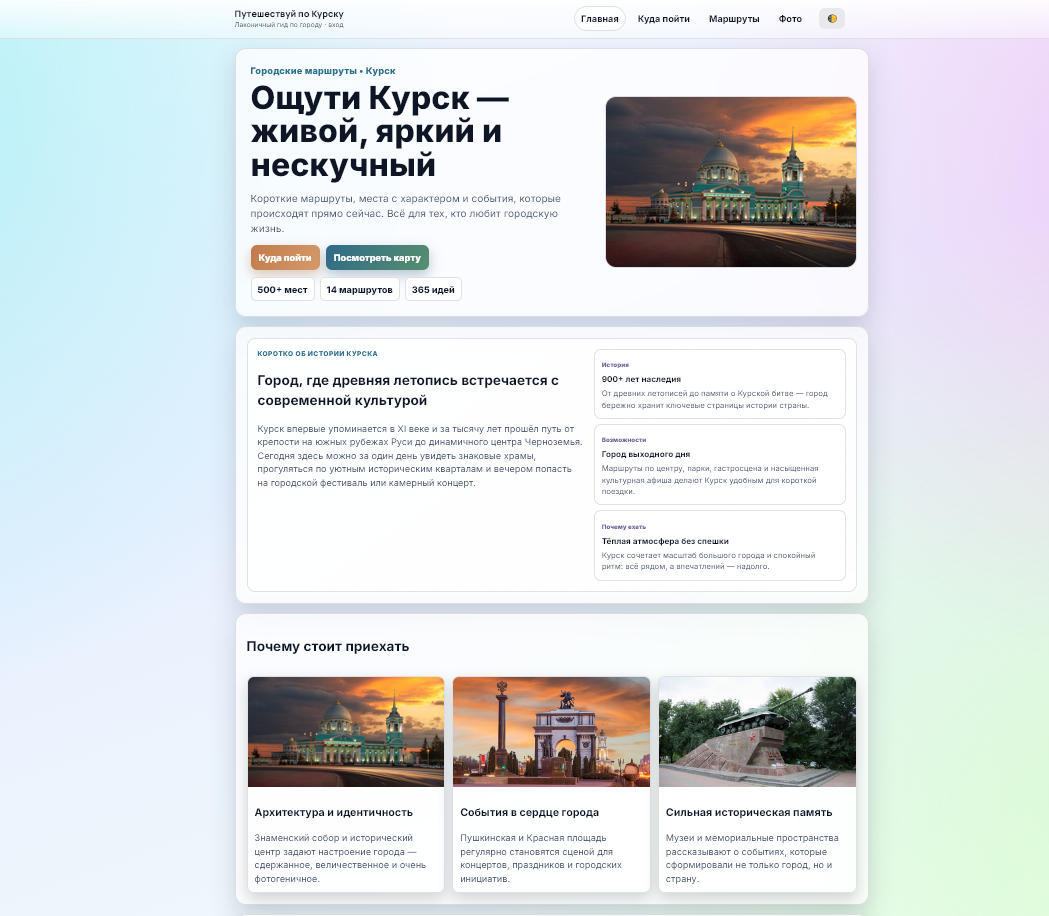
\includegraphics[width=0.8\linewidth]{images/ui-main}
	\caption{Главная страница веб-приложения}
	\label{fig:ui-main}
\end{figure}

Как показано на рисунке, главная страница содержит шапку с названием
системы и навигацией по разделам, блоки описания проекта, а также карту с
маркерами объектов. Каркас интерфейса одинаков для всех пользовательских
страниц, что снижает порог входа и ускоряет навигацию.

Окно просмотра карточки объекта показано на рисунке~\ref{fig:ui-modal-object}.

\begin{figure}[H]
	\centering
	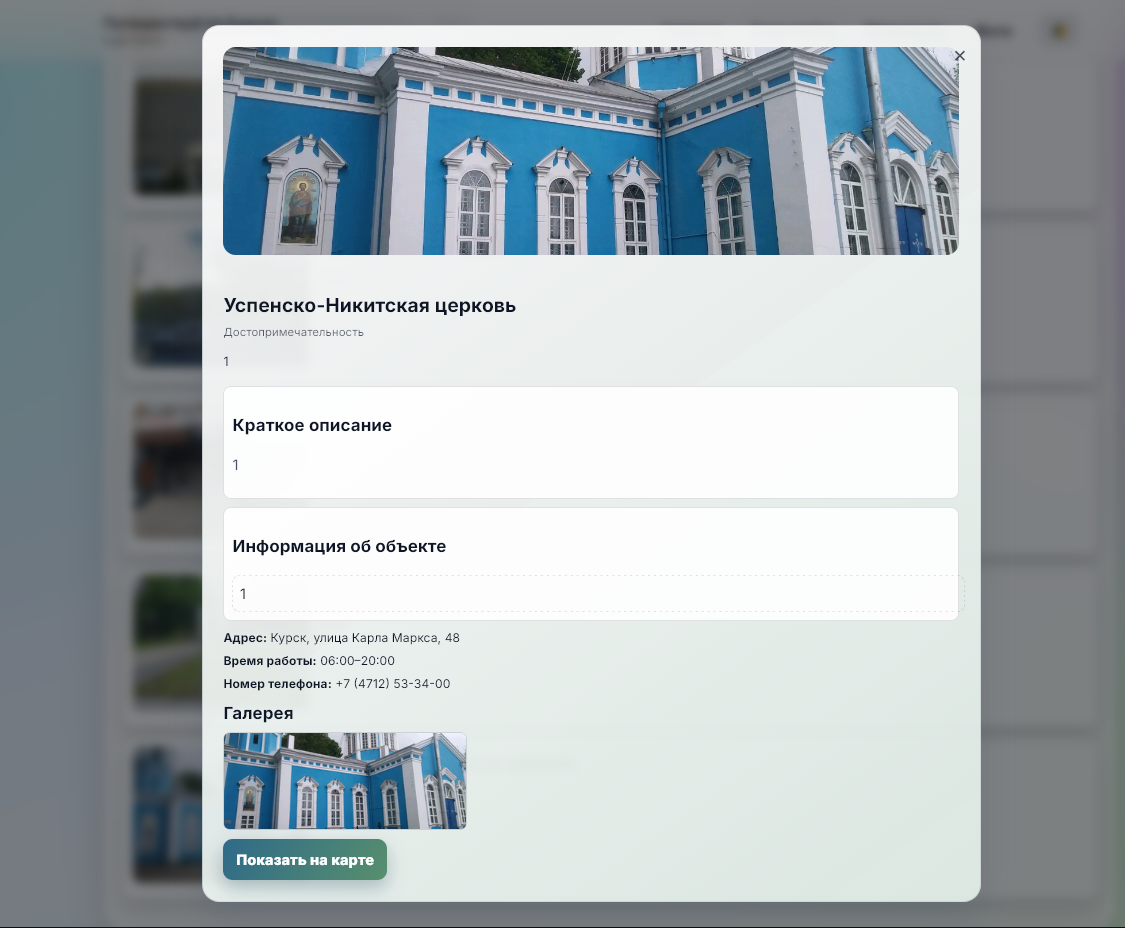
\includegraphics[width=0.8\linewidth]{images/ui-modal-object}
	\caption{Окно просмотра подробной информации об объекте}
	\label{fig:ui-modal-object}
\end{figure}

Окно просмотра карточки маршрута показано на рисунке~\ref{fig:ui-modal-route}.

\begin{figure}[H]
	\centering
	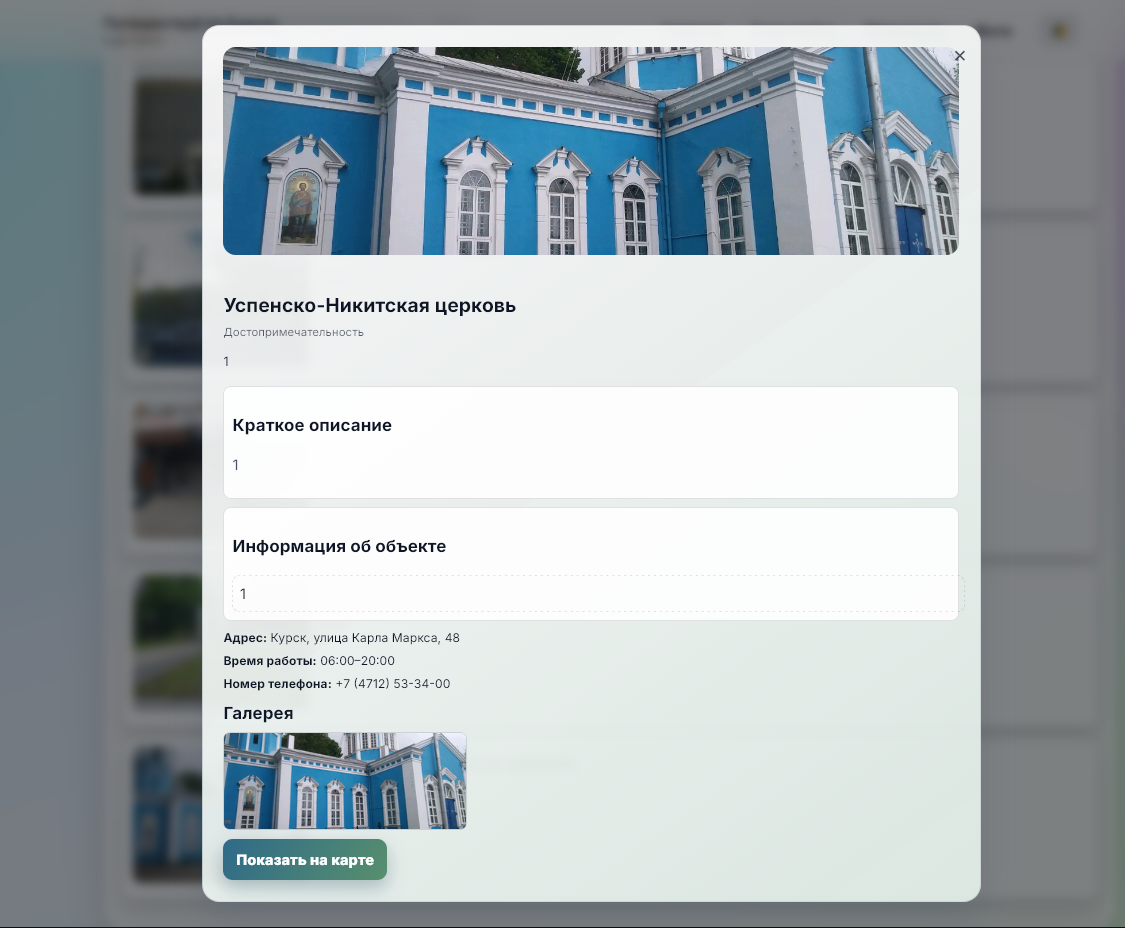
\includegraphics[width=0.8\linewidth]{images/ui-modal-object}
	\caption{Окно просмотра подробной информации о маршруте}
	\label{fig:ui-modal-route}
\end{figure}

\subsection{Моделирование вариантов использования}
В системе выделяются два действующих лица:
\begin{enumerate}
	\item Пользователь --- просматривает опубликованный контент.
	\item Администратор --- управляет контентом системы.
\end{enumerate}

Далее приведены агрегированные перечни прецедентов для каждой роли; они детализируются в последующих подпунктах.

Перечень прецедентов пользователя:
\begin{enumerate}
	\item Просмотреть главную страницу.
	\item Просмотреть карту с маркерами.
	\item Просмотреть список мест.
	\item Отфильтровать места по категории.
	\item Открыть карточку места.
	\item Перейти к месту на карте.
	\item Просмотреть список маршрутов.
	\item Открыть карточку маршрута.
	\item Просмотреть фото-галерею.
	\item Открыть фото в модальном окне.
	\item Открыть связанное место из фото.
\end{enumerate}

\begin{figure}[H]
	\centering
	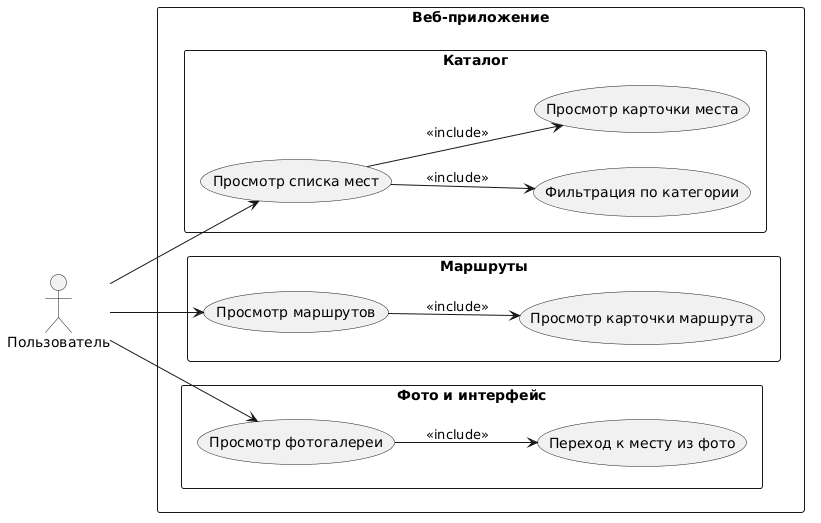
\includegraphics[width=0.8\linewidth]{images/usecase-user}
	\caption{Диаграмма прецедентов для пользователя}
	\label{fig:usecase-user}
\end{figure}

Перечень прецедентов администратора:
\begin{enumerate}
	\item Добавить категорию.
	\item Добавить объект.
	\item Редактировать объект.
	\item Удалить объект.
	\item Опубликовать/скрыть объект.
	\item Выбрать координаты объекта на карте.
	\item Просмотреть список объектов.
	\item Добавить маршрут.
	\item Редактировать маршрут.
	\item Удалить маршрут.
	\item Добавить/удалить/переставить точки маршрута.
	\item Опубликовать/скрыть маршрут.
	\item Просмотреть список маршрутов.
\end{enumerate}

\begin{figure}[H]
	\centering
	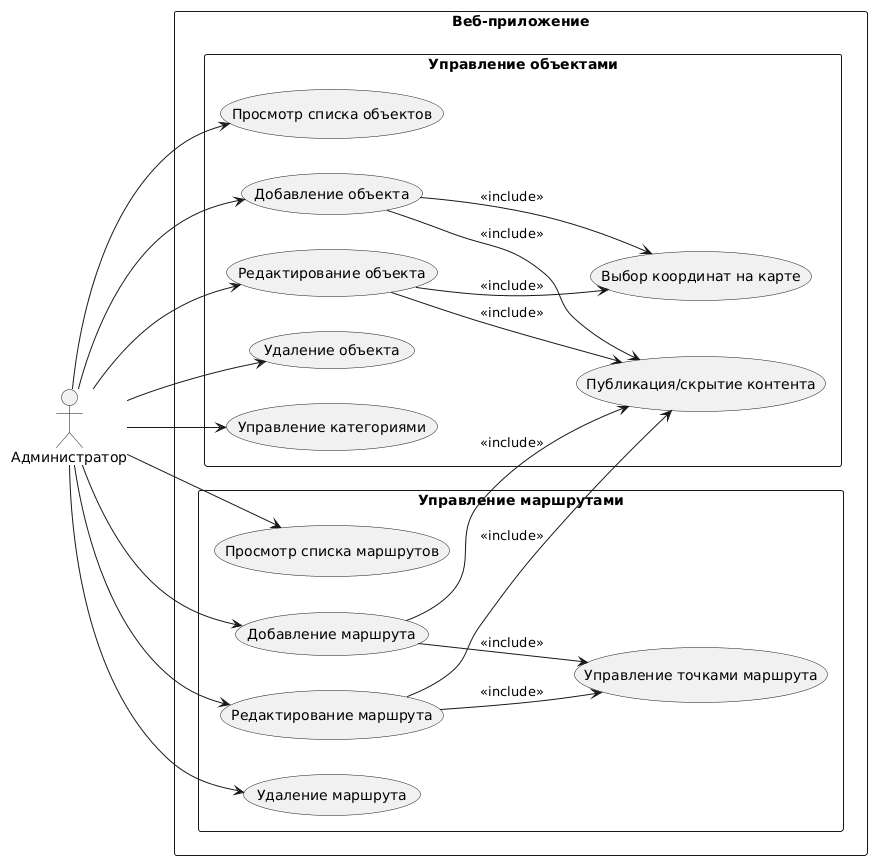
\includegraphics[width=0.8\linewidth]{images/usecase-admin}
	\caption{Диаграмма прецедентов использования для администратора}
	\label{fig:usecase-admin}
\end{figure}

\subsubsection{Вариант использования «Просмотр списка мест»}
\textbf{Заинтересованные лица и их требования:} пользователь желает увидеть доступные места города.

\textbf{Предусловие:} открыта страница «Куда пойти».

\textbf{Постусловие:} отображён список опубликованных объектов.

\textbf{Основной успешный сценарий:}
\begin{enumerate}
	\item Пользователь открывает страницу «Куда пойти».
	\item Система запрашивает категории и опубликованные места через API.
	\item Система формирует карточки мест.
	\item Пользователь просматривает список.
\end{enumerate}

\subsubsection{Вариант использования «Фильтрация мест по категории»}
\textbf{Заинтересованные лица и их требования:} пользователь желает быстро отобрать места по интересующей категории.

\textbf{Предусловие:} список мест загружен, доступны кнопки/элементы фильтрации по категориям.

\textbf{Постусловие:} отображаются только места выбранной категории.

\textbf{Основной успешный сценарий:}
\begin{enumerate}
	\item Пользователь выбирает категорию.
	\item Система применяет фильтр к текущему набору мест.
	\item Карточки в списке обновляются.
\end{enumerate}

\textbf{Альтернативный сценарий (пустой результат):}
\begin{enumerate}
	\item В желаемой категории отсутствуют места.
	\item Система не даёт возможность выбрать категорию.
\end{enumerate}

\subsubsection{Вариант использования «Просмотр карточки места»}
\textbf{Заинтересованные лица и их требования:} пользователь желает получить подробную информацию о конкретном месте.

\textbf{Предусловие:} место отображается в списке или на карте.

\textbf{Постусловие:} открыто модальное окно с детальной информацией о месте.

\textbf{Основной успешный сценарий:}
\begin{enumerate}
	\item Пользователь выбирает карточку места (или маркер на карте).
	\item Система открывает модальное окно.
	\item Отображаются название, описание, контакты, адрес, галерея и ссылки.
\end{enumerate}

\textbf{Альтернативный сценарий (неполные данные):}
\begin{enumerate}
	\item У места отсутствуют часть полей (например, сайт/телефон).
	\item Система скрывает или оставляет пустыми отсутствующие поля.
\end{enumerate}

\subsubsection{Вариант использования «Просмотр мест на карте»}
\textbf{Заинтересованные лица и их требования:} пользователь желает видеть пространственное расположение мест.

\textbf{Предусловие:} открыта главная страница, карта загружена.

\textbf{Постусловие:} пользователь видит маркеры мест и может с ними взаимодействовать.

\textbf{Основной успешный сценарий:}
\begin{enumerate}
	\item Пользователь переходит к блоку карты.
	\item Система отображает карту и маркеры опубликованных мест.
	\item Пользователь кликает по маркеру.
	\item Система открывает карточку соответствующего места.
\end{enumerate}

\subsubsection{Вариант использования «Просмотр списка маршрутов»}
\textbf{Заинтересованные лица и их требования:} пользователь желает получить готовые маршруты прогулок.

\textbf{Предусловие:} открыта страница «Маршруты».

\textbf{Постусловие:} отображён список опубликованных маршрутов.

\textbf{Основной успешный сценарий:}
\begin{enumerate}
	\item Пользователь открывает страницу «Маршруты».
	\item Система запрашивает список маршрутов через API.
	\item Система выводит маршруты в интерфейсе.
\end{enumerate}

\textbf{Альтернативный сценарий (маршрутов нет):} 
\begin{enumerate}
	\item В базе отсутствуют опубликованные маршруты.
	\item Система отображает пустой список.
\end{enumerate}

\subsubsection{Вариант использования «Просмотр карточки маршрута»}
\textbf{Заинтересованные лица и их требования:} пользователь желает получить подробный состав маршрута.

\textbf{Предусловие:} маршрут присутствует в списке.

\textbf{Постусловие:} открыто окно маршрута со списком точек и картой.

\textbf{Основной успешный сценарий:}
\begin{enumerate}
	\item Пользователь выбирает маршрут.
	\item Система открывает модальное окно маршрута.
	\item Отображаются описание и точки маршрута.
	\item Маршрут визуализируется на карте.
\end{enumerate}

\subsubsection{Вариант использования «Просмотр фотогалереи»}
\textbf{Заинтересованные лица и их требования:} пользователь желает просмотреть фото мест города.

\textbf{Предусловие:} открыта страница «Фото».

\textbf{Постусловие:} отображена сетка изображений.

\textbf{Основной успешный сценарий:}
\begin{enumerate}
	\item Пользователь открывает страницу «Фото».
	\item Система формирует галерею из доступных изображений.
	\item Пользователь просматривает сетку фото.
\end{enumerate}

\subsubsection{Вариант использования «Открытие фото в модальном окне»}
\textbf{Заинтересованные лица и их требования:} пользователь желает рассмотреть фото в увеличенном виде.

\textbf{Предусловие:} фото отображается в галерее.

\textbf{Постусловие:} открыто модальное окно с увеличенным изображением.

\textbf{Основной успешный сценарий:}
\begin{enumerate}
	\item Пользователь нажимает на фото.
	\item Система открывает модальное окно.
	\item Отображаются увеличенное фото и действия для дальнейшего перехода.
\end{enumerate}

\subsubsection{Вариант использования «Переход к месту из фото»}
\textbf{Заинтересованные лица и их требования:} пользователь желает перейти от фото к карточке конкретного места.

\textbf{Предусловие:} открыто модальное окно фото.

\textbf{Постусловие:} открыта карточка связанного места.

\textbf{Основной успешный сценарий:}
\begin{enumerate}
	\item Пользователь нажимает кнопку «Что это за место?».
	\item Система определяет связанный объект.
	\item Система открывает карточку места.
\end{enumerate}

\subsubsection{Вариант использования «Вход в панель администратора»}
\textbf{Заинтересованные лица и их требования:} администратор желает получить доступ к функциям управления контентом.

\textbf{Предусловие:} открыта страница администрирования, доступ к панели не подтверждён.

\textbf{Постусловие:} администратор получает доступ к функциям управления объектами и маршрутами.

\textbf{Основной успешный сценарий:}
\begin{enumerate}
	\item Администратор открывает страницу панели.
	\item Система запрашивает подтверждение доступа.
	\item Администратор вводит учётные данные.
	\item Доступ подтверждается.
	\item Отображается интерфейс управления объектами и маршрутами.
\end{enumerate}

\textbf{Альтернативный сценарий (неверные данные доступа):} 
\begin{enumerate}
	\item Администратор вводит неверные данные.
	\item Система отображает отказ в доступе.
	\item Страница управления не открывается.
\end{enumerate}

\subsubsection{Вариант использования «Добавление категории»}
\textbf{Заинтересованные лица и их требования:} администратор желает расширить классификацию объектов.

\textbf{Предусловие:} открыта панель администратора.

\textbf{Постусловие:} новая категория сохранена и доступна в выпадающих списках.

\textbf{Основной успешный сценарий:}
\begin{enumerate}
	\item Администратор вводит название новой категории.
	\item Нажимает кнопку добавления категории.
	\item Система сохраняет категорию в базе данных.
	\item Система обновляет список категорий в форме объекта.
\end{enumerate}

\textbf{Альтернативный сценарий (пустое значение):}
\begin{enumerate}
	\item Администратор оставляет поле категории пустым.
	\item Сохранение не выполняется.
\end{enumerate}

\subsubsection{Вариант использования «Добавление объекта»}
\textbf{Заинтересованные лица и их требования:} администратор желает создать новую карточку места.

\textbf{Предусловие:} открыта панель администратора, загружены категории.

\textbf{Постусловие:} объект сохранён в базе и отображается в списке объектов.

\textbf{Основной успешный сценарий:}
\begin{enumerate}
	\item Администратор заполняет форму объекта.
	\item Нажимает «Сохранить объект».
	\item Система валидирует поля.
	\item Система отправляет данные в API и сохраняет объект.
	\item Список объектов обновляется.
\end{enumerate}

\textbf{Альтернативный сценарий (ошибка валидации):} 
\begin{enumerate}
	\item Обнаружены некорректные или пустые обязательные поля.
	\item Система выводит список ошибок.
	\item Объект не сохраняется.
\end{enumerate}

\subsubsection{Вариант использования «Редактирование объекта»}
\textbf{Заинтересованные лица и их требования:} администратор желает обновить данные существующего объекта.

\textbf{Предусловие:} объект присутствует в списке панели администратора.

\textbf{Постусловие:} обновлённые данные сохранены в базе.

\textbf{Основной успешный сценарий:}
\begin{enumerate}
	\item Администратор нажимает «Редактировать» для выбранного объекта.
	\item Система подставляет текущие данные в форму.
	\item Администратор меняет значения и сохраняет изменения.
	\item Система обновляет объект в базе данных.
\end{enumerate}

\subsubsection{Вариант использования «Удаление объекта»}
\textbf{Заинтересованные лица и их требования:} администратор желает удалить неактуальный объект.

\textbf{Предусловие:} объект существует в базе данных.

\textbf{Постусловие:} объект удалён, список объектов обновлён.

\textbf{Основной успешный сценарий:}
\begin{enumerate}
	\item Администратор выбирает действие «Удалить».
	\item Система выполняет запрос удаления.
	\item Объект удаляется из базы.
	\item Система обновляет список объектов.
\end{enumerate}

\subsubsection{Вариант использования «Выбор координат объекта на карте»}
\textbf{Заинтересованные лица и их требования:} администратор желает точно указать координаты объекта.

\textbf{Предусловие:} открыта форма объекта в панели администратора.

\textbf{Постусловие:} поля широты и долготы заполнены выбранными координатами.

\textbf{Основной успешный сценарий:}
\begin{enumerate}
	\item Администратор открывает модальное окно выбора координат.
	\item Система загружает карту.
	\item Администратор кликает по карте.
	\item Система показывает подтверждение подстановки координат.
	\item После подтверждения координаты переносятся в форму.
\end{enumerate}

\subsubsection{Вариант использования «Добавление маршрута»}
\textbf{Заинтересованные лица и их требования:} администратор желает создать новый маршрут.

\textbf{Предусловие:} в системе есть доступные объекты для выбора точек маршрута.

\textbf{Постусловие:} маршрут сохранён и отображается в списке маршрутов.

\textbf{Основной успешный сценарий:}
\begin{enumerate}
	\item Администратор заполняет название и описание маршрута.
	\item Добавляет минимум две точки маршрута.
	\item Нажимает «Сохранить маршрут».
	\item Система валидирует структуру маршрута.
	\item Система сохраняет маршрут и связанные точки.
\end{enumerate}

\textbf{Альтернативный сценарий (меньше двух точек):} 
\begin{enumerate}
	\item Администратор пытается сохранить маршрут с одной или нулём точек.
	\item Система выводит ошибку валидации.
	\item Маршрут не сохраняется.
\end{enumerate}

\subsubsection{Вариант использования «Редактирование маршрута»}
\textbf{Заинтересованные лица и их требования:} администратор желает изменить параметры существующего маршрута.

\textbf{Предусловие:} маршрут существует в базе данных.

\textbf{Постусловие:} изменения маршрута сохранены.

\textbf{Основной успешный сценарий:}
\begin{enumerate}
	\item Администратор выбирает маршрут в списке.
	\item Система загружает данные маршрута в форму.
	\item Администратор изменяет описание, видимость или точки.
	\item Сохраняет изменения.
	\item Система обновляет маршрут.
\end{enumerate}

\subsubsection{Вариант использования «Удаление маршрута»}
\textbf{Заинтересованные лица и их требования:} администратор желает удалить неактуальный маршрут.

\textbf{Предусловие:} маршрут присутствует в списке маршрутов.

\textbf{Постусловие:} маршрут удалён из базы данных.

\textbf{Основной успешный сценарий:}
\begin{enumerate}
	\item Администратор нажимает «Удалить маршрут».
	\item Система отправляет запрос на удаление.
	\item Маршрут удаляется.
	\item Список маршрутов обновляется.
\end{enumerate}

\subsubsection{Вариант использования «Управление точками маршрута»}
\textbf{Заинтересованные лица и их требования:} администратор желает настроить последовательность прохождения маршрута.

\textbf{Предусловие:} открыта форма добавления/редактирования маршрута.

\textbf{Постусловие:} точки маршрута сохранены в актуальном порядке.

\textbf{Основной успешный сценарий:}
\begin{enumerate}
	\item Администратор добавляет точки из списка доступных объектов.
	\item При необходимости удаляет лишние точки.
	\item Меняет порядок точек кнопками «вверх/вниз».
	\item Система визуально обновляет последовательность.
	\item При сохранении маршрута порядок записывается в базу данных.
\end{enumerate}

\subsubsection{Вариант использования «Управление публикацией контента»}
\textbf{Заинтересованные лица и их требования:} администратор желает контролировать видимость объектов и маршрутов в пользовательской части.

\textbf{Предусловие:} открыт режим редактирования объекта или маршрута.

\textbf{Постусловие:} признак видимости (published/hidden) сохранён.

\textbf{Основной успешный сценарий:}
\begin{enumerate}
	\item Администратор устанавливает/снимает флаг публикации.
	\item Сохраняет изменения.
	\item Система обновляет запись в базе.
	\item Контент появляется или скрывается в пользовательских разделах.
\end{enumerate}

\subsection{Требования к надёжности}
Система должна обеспечивать надёжную обработку и хранение данных как при
обычной эксплуатации, так и при возникновении ошибок.

\textbf{Целостность данных.} Операции создания и обновления маршрутов
выполняются в транзакциях PostgreSQL, что исключает сохранение частично
заполненных маршрутов (например, при ошибке между сохранением маршрута и
сохранением его точек).

\textbf{Устойчивость API.} Серверная часть должна корректно обрабатывать
ошибки и возвращать стандартизированные ответы JSON с кодами HTTP 4xx/5xx
без аварийного завершения процесса Node.js.

\textbf{Валидация входных данных.} На стороне клиентского административного
интерфейса и на стороне API должна выполняться проверка обязательных полей
(название, категория, координаты, структура маршрута), чтобы предотвратить
попадание некорректных записей в базу данных.

\textbf{Логирование ошибок.} Ошибки API должны фиксироваться в журнале
приложения (stdout/stderr или файл логов окружения), включая текст ошибки и
контекст запроса для последующей диагностики.

\textbf{Резервное копирование.} Для обеспечения сохранности данных должно
выполняться регулярное резервное копирование базы PostgreSQL штатными
средствами (pg\_dump/pg\_restore) или средствами инфраструктуры.

\subsection{Требования к информационной безопасности}
Система должна обеспечивать защиту данных и административного контура от
несанкционированного доступа.

\textbf{Разграничение доступа к админ-разделу.} Доступ к
странице \texttt{/pages/admin.html} должен ограничиваться на уровне
инфраструктуры.

\textbf{Защита от SQL-инъекций.} Все обращения к базе данных должны
выполняться через параметризованные SQL-запросы.

\textbf{Валидация пользовательского ввода.} Все текстовые и URL-поля,
передаваемые через API, должны проверяться на корректность формата и длины
для предотвращения передачи вредоносных или некорректных данных.

\textbf{Защита административных операций.} Действия удаления и публикации
контента должны выполняться только через административный интерфейс и
журналироваться средствами сервера/инфраструктуры.

\subsection{Требования к программной и технической совместимости}
Система должна корректно функционировать в типовой среде разработки и
развёртывания веб-приложений.

\textbf{Операционная система сервера.} Серверная часть должна работать в
средах Linux, Windows и macOS при наличии Node.js и PostgreSQL совместимых
версий.

\textbf{Программные зависимости.} Для работы приложения необходимы:
Node.js, пакетный менеджер npm, СУБД PostgreSQL, а также доступ к внешнему
скрипту Yandex Maps API.

\textbf{Требования к браузеру.} Клиентская часть должна корректно
отображаться в актуальных версиях Google Chrome, Mozilla Firefox,
Microsoft Edge и других современных браузерах с поддержкой ES6.

\textbf{Совместимость данных.} Приложение должно работать с БД PostgreSQL,
содержащей таблицы \texttt{categories}, \texttt{places}, \texttt{routes},
\texttt{route\_points}.

\subsection{Требования к оформлению документации}
Разработка программной документации и программного изделия должна производиться согласно ГОСТ 19.102-77 и ГОСТ 34.601-90. Единая система программной документации.
